\begin{figure*}[t]
  \centering
  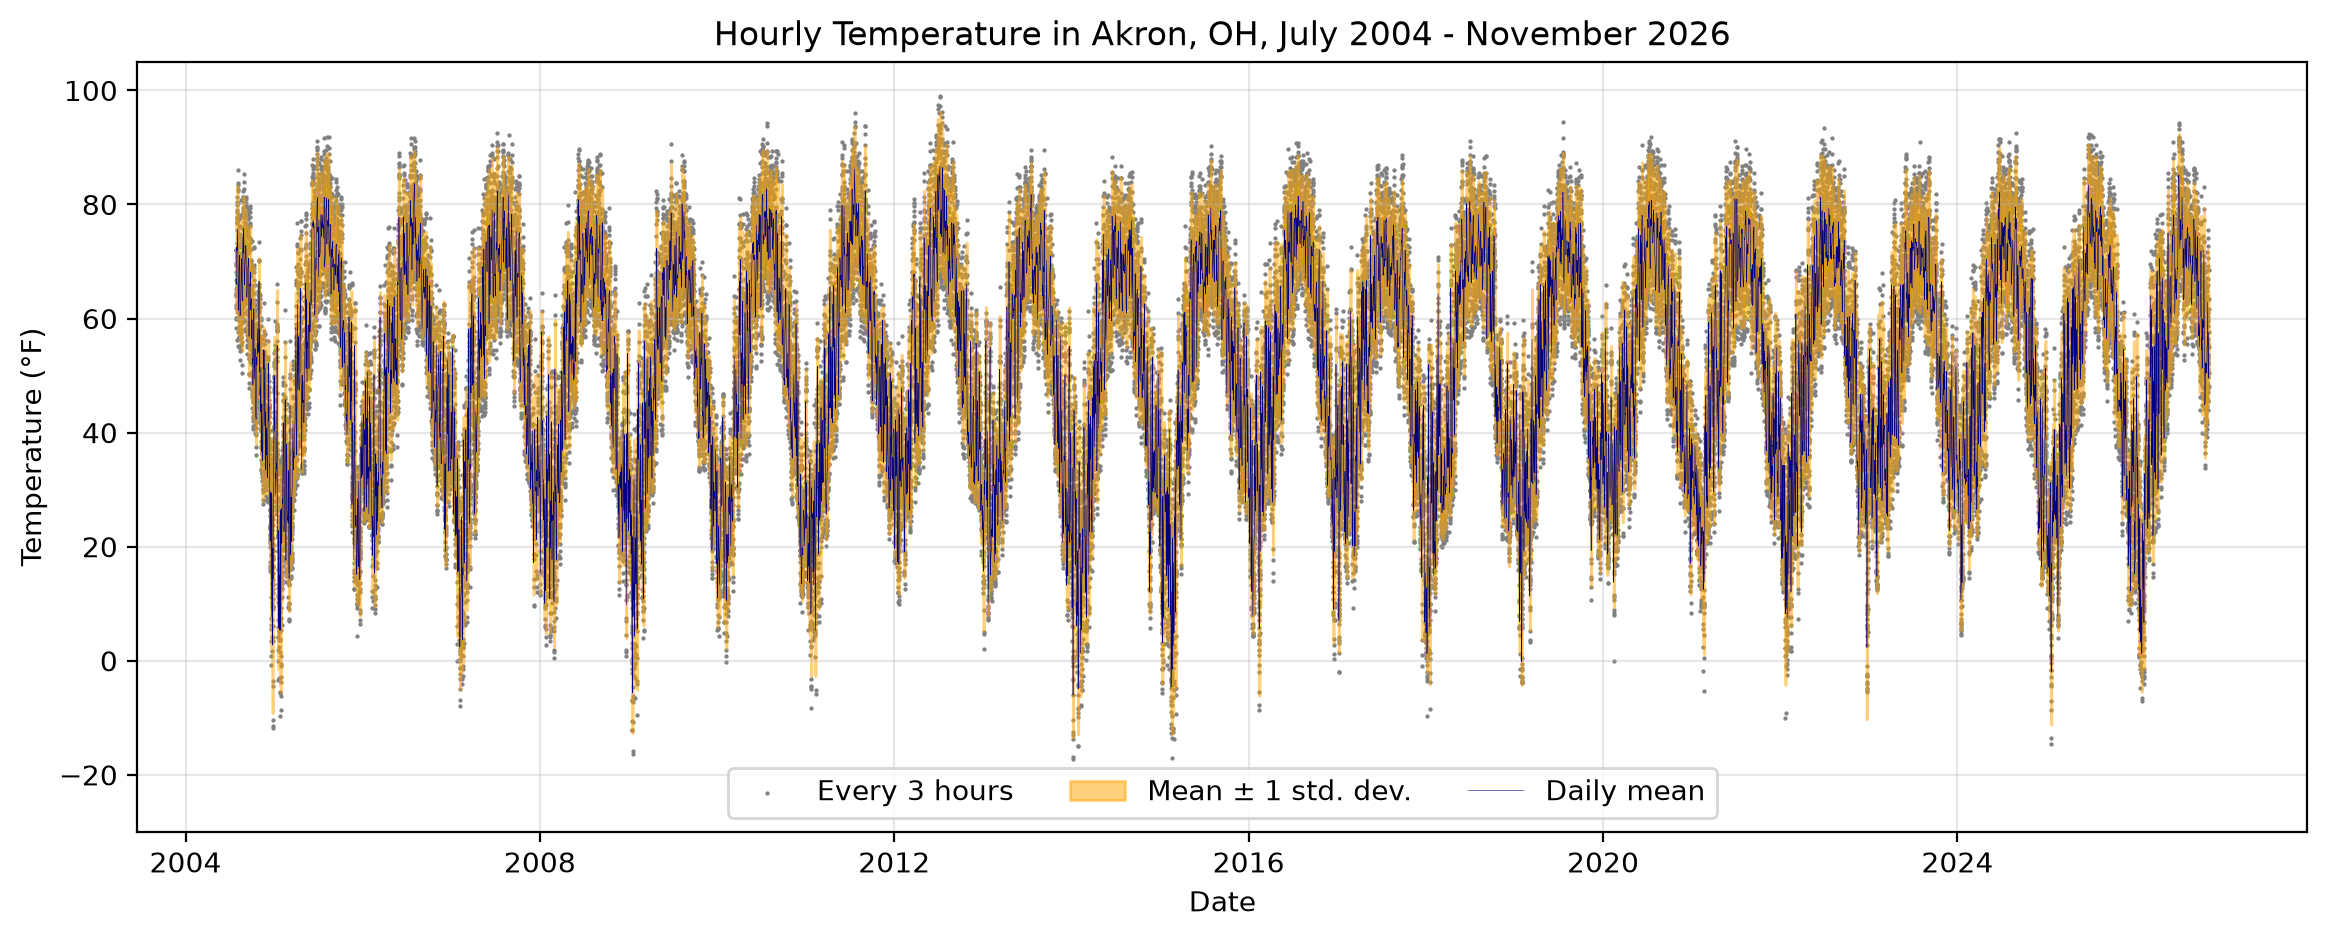
\includegraphics[width=\textwidth,height=0.23\textheight,keepaspectratio]{temperature_full.png}
  \caption{\label{fig:full} Hourly temperature in Akron, OH, July
    2004--November 2026. 
    Gray dots: readings every 3 hours. 
    Blue line:
    daily mean. 
    Orange band: daily mean $\pm$ 1 standard deviation.}
\end{figure*}

\begin{figure*}[t]
  \centering
  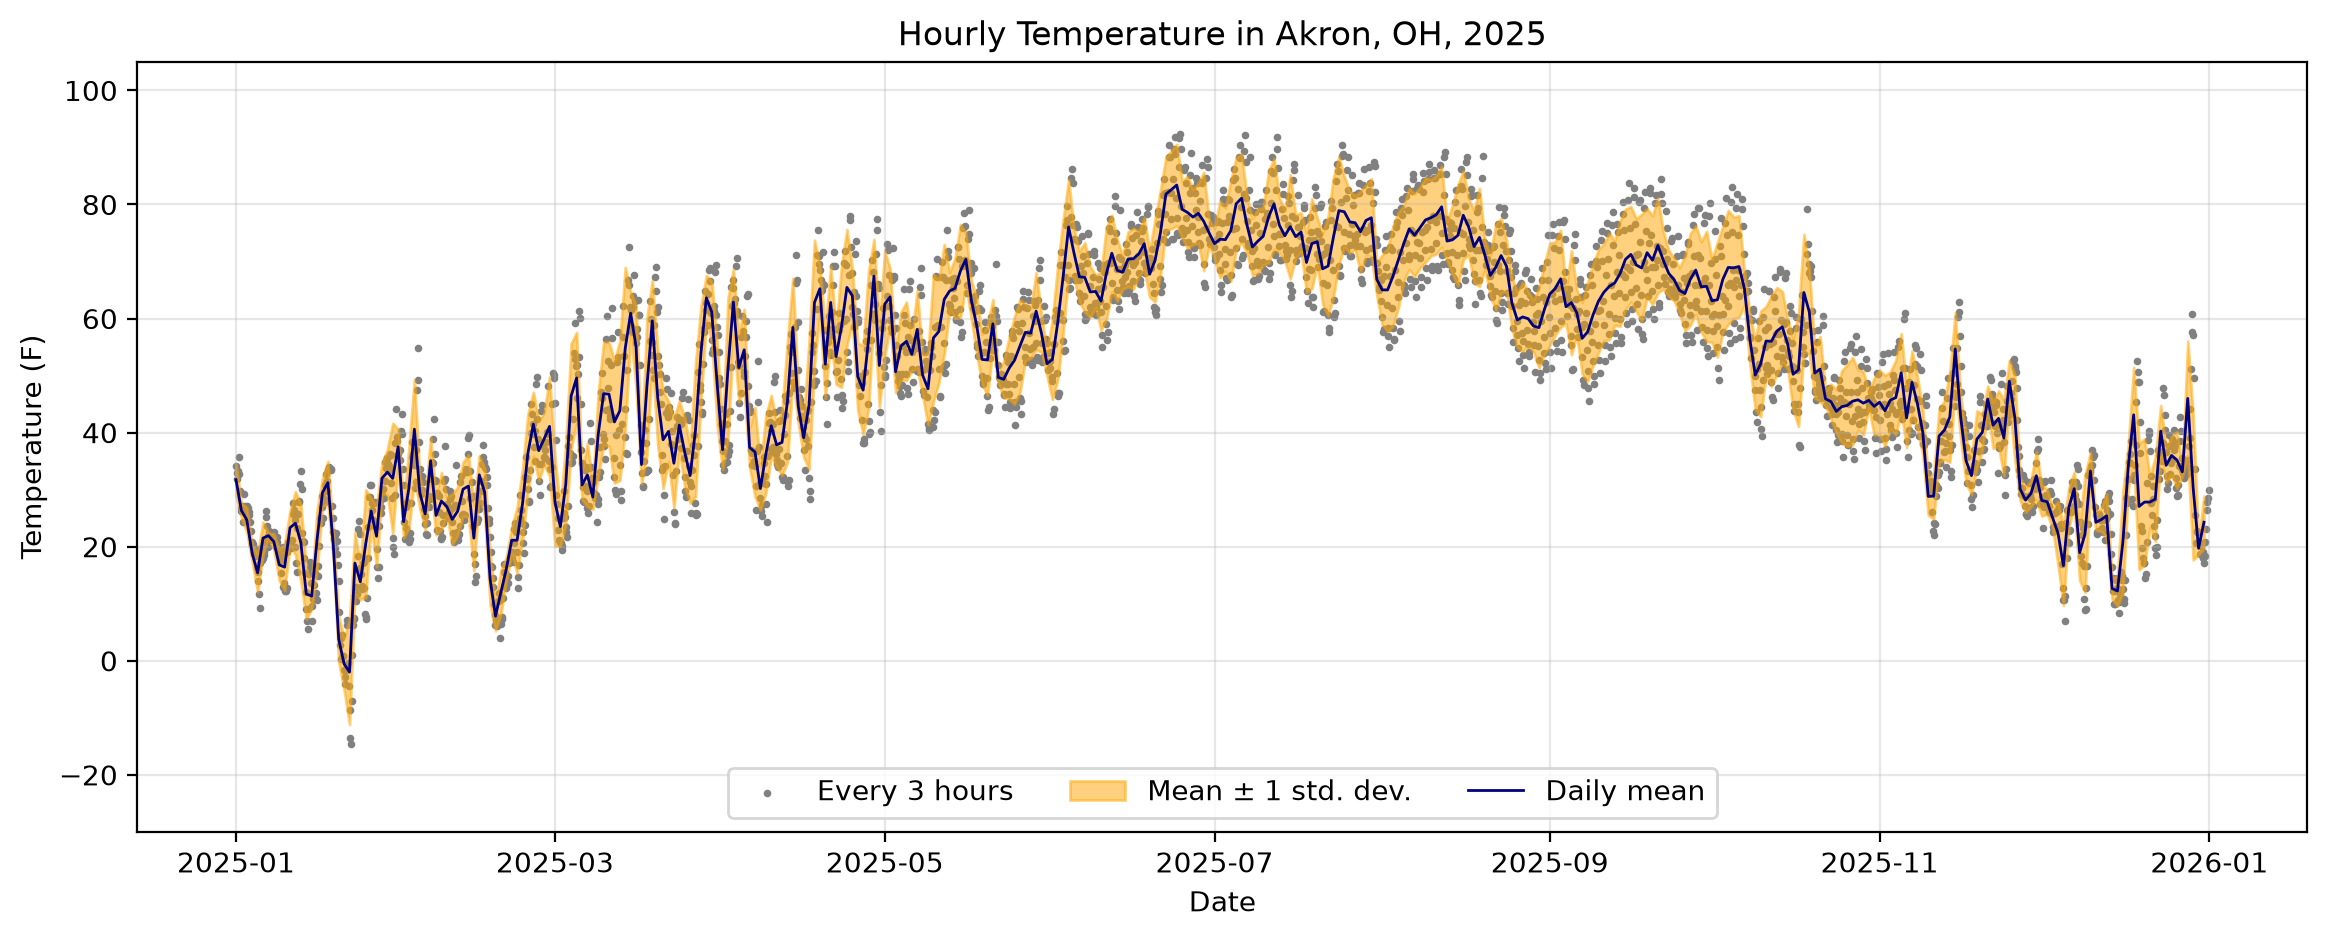
\includegraphics[width=\textwidth,height=0.23\textheight,keepaspectratio]{temperature_2025.png}
  \caption{\label{fig:year} Hourly temperature in Akron, OH, during 2025. 
    Gray dots: readings every 3 hours. 
    Blue line: daily mean. 
    Orange band: daily mean $\pm$ 1 standard deviation.}
\end{figure*}

\begin{figure*}[t]
  \centering
  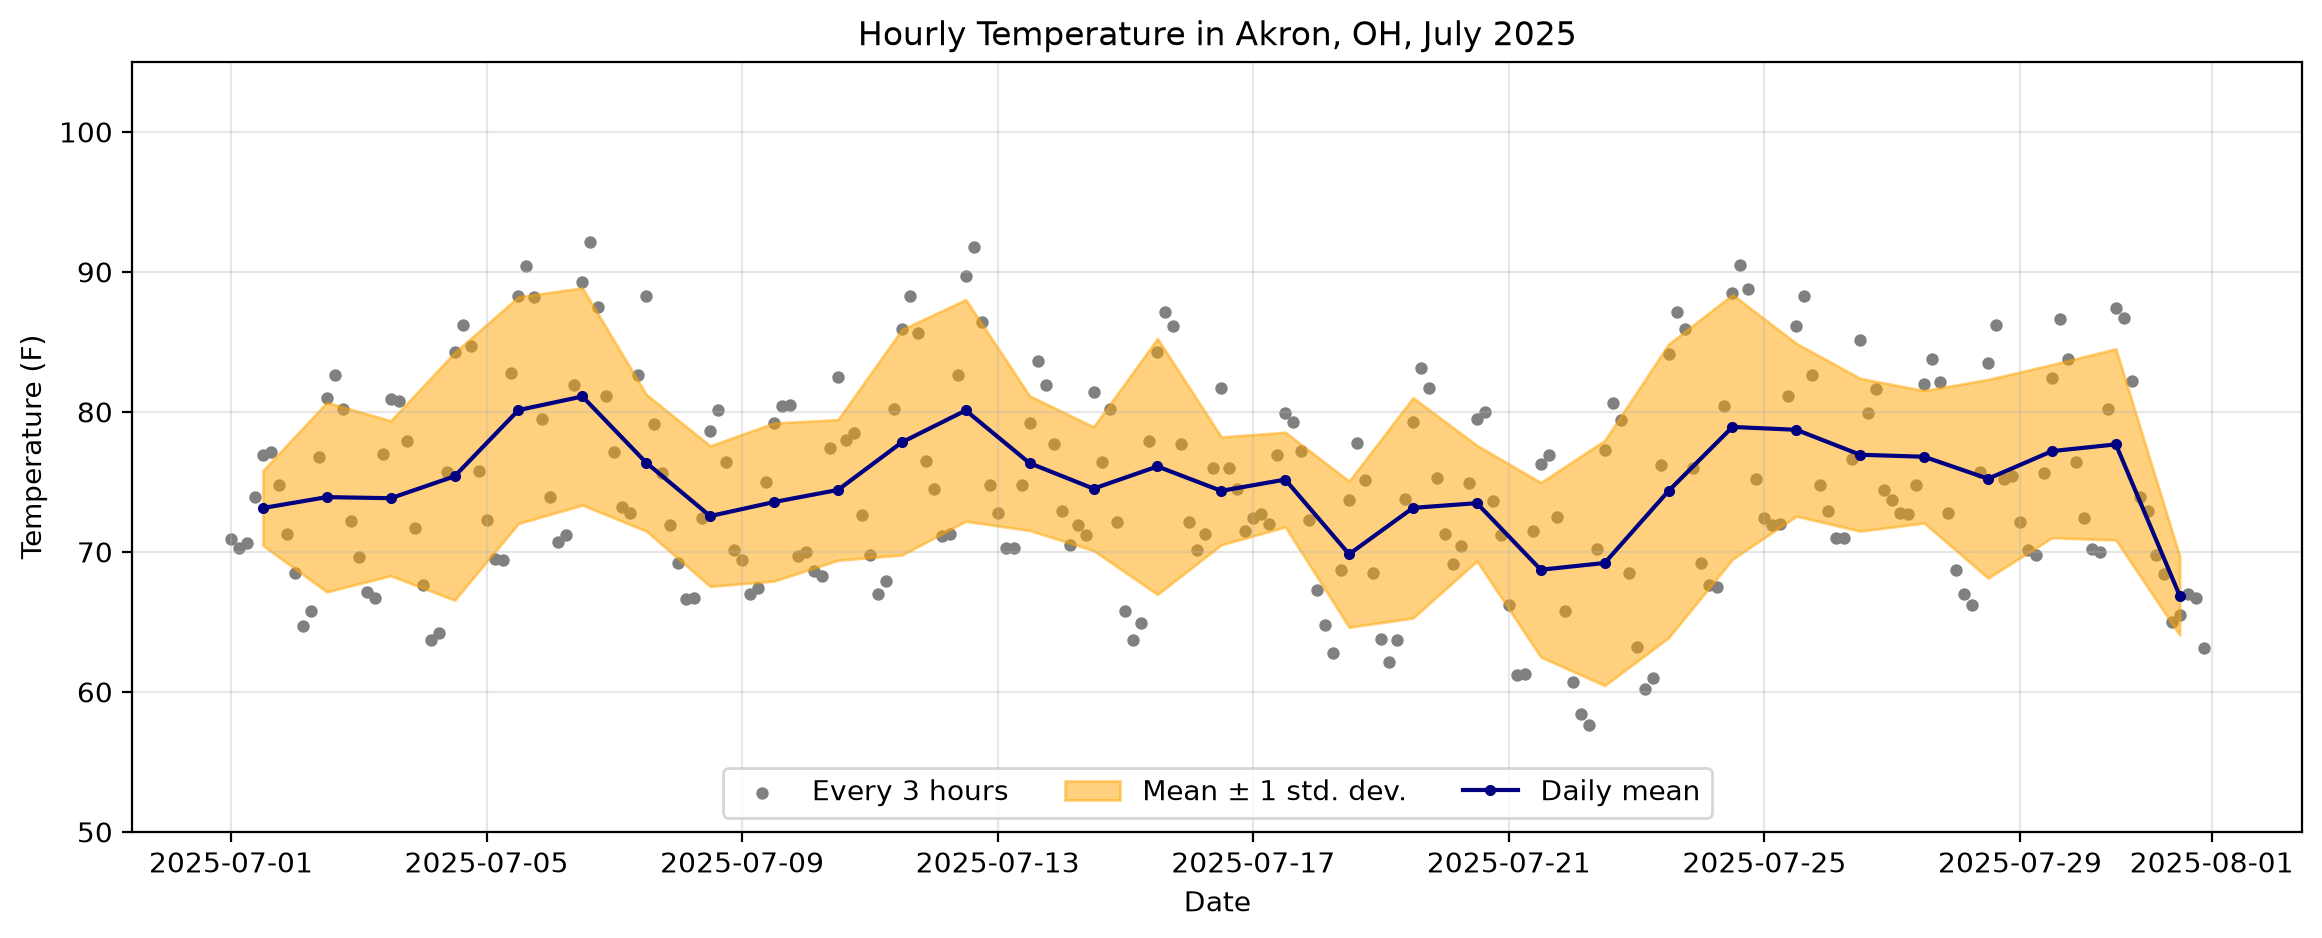
\includegraphics[width=\textwidth,height=0.23\textheight,keepaspectratio]{temperature_month.png}
  \caption{\label{fig:month} Hourly temperature in Akron, OH, during July
    2025.
    Gray dots: readings every 3 hours. 
    Blue line: daily mean. 
    Orange band: daily mean $\pm$ 1 standard deviation.}
\end{figure*}

I plotted the temperature data at three different scales, the full 22 year record, the entire 2025 year, and one month. In every figure, the gray dots are the raw readings every 3 hours, the blue line  is the daily mean (Equation~\ref{eq:mean}), and the orange band is the daily mean plus or minus  one standard deviation (Equation~\ref{eq:std}).

Figure~\ref{fig:full} shows the full 22 year record. The seasonly cycle is shown through the temperature rising to its peak each summer and drops to its lowest point each winter. Since 22 years are squeezed into  one plot, the details are hard to see, so the next figures zoom in.

Figure~\ref{fig:year} shows the entire year of 2025. At this scale, the spread of the gray dots around the daily mean is visible, and so is the day-to-day noise caused by passing weather systems.

Figure~\ref{fig:month} zooms in to July 2025. Each day now has its own step in the navy line and its own  section of the orange band. A tall band means a large standard deviation, so the temperature changed a lot that day. A short band means the temperature stayed steady.